\section{Einstieg}

\begin{frame}{Problemstellung}
	\begin{itemize}
		\item Punkte gleichmäßig im Raum verteilen
		\item Mehrere existierende Verfahren
		\begin{itemize}
			\item Halton
			\item Blue noise
		\end{itemize}
		\item \textbf{Ziel 1}: effizientes Vorgehen 
		\item \textbf{Ziel 2}: mehrdimensional anwendbar
		\item \textbf{Ziel 3}: unabhängig von bestimmten Eigenschaften der Funktion einsetzbar
	\end{itemize}
\end{frame}

\begin{frame}{Ziel}
	\begin{figure}
		\begin{subfigure}{.45\textwidth}
			\centering
			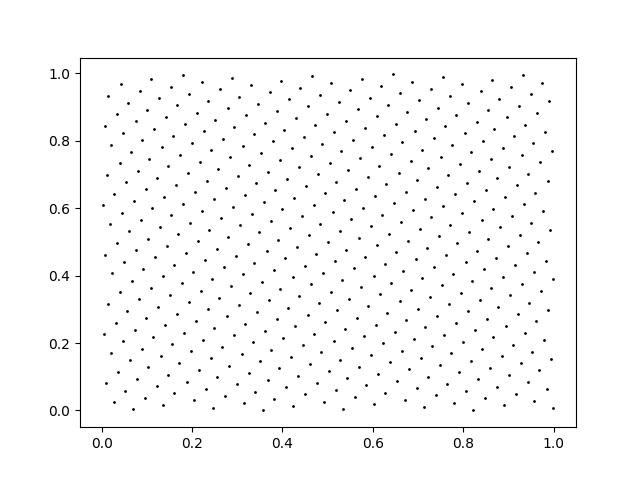
\includegraphics[width=\textwidth]{pdf_plots/grs_u500c.pdf}
		\end{subfigure}
		% \hfill
		% \begin{subfigure}{.15\textwidth}
		% 	\centering
		% 	
\includegraphics[width=.5\textwidth, angle=180]{Screenshots/img_71815.png}
		% \end{subfigure}
		% \hfill
		\begin{subfigure}{.45\textwidth}
			\centering
			\includegraphics[width=\textwidth]{pdf_plots/idf2_log-log_iu500c-GRS.pdf}
		\end{subfigure}
	\end{figure}
\end{frame}